\section{Töövahendid}


\textbf{Python}

Python on üldotstarbeline programmeerimiskeel, mida kasutatakse
laialdaselt andmeteaduse, masinõppe ja ruumiandmete analüüsi ülesanneteks
oma lihtsuse ja mitmekülgsuse tõttu.



\textbf{Jupyter Notebookid}\nopagebreak[4]

Jupyter Notebookid pakuvad interaktiivset keskkonda, kus
saab koodi kirjutada, käivitada ja dokumenteerida ühes kohas. Need võimaldavad
dünaamilist andmeanalüüsi ja tulemuste visuaalset esitlust, muutes
uurimisprotsessi läbipaistvaks ja korduvaks.



\textbf{Pandas}\nopagebreak[4]

Pandas on andmetöötluse teek, mis pakub paindlikke ja
efektiivseid andmestruktuure tabelipõhise andmetöötluse jaoks. See lihtsustab
andmete puhastamist, analüüsi ja manipuleerimist.


\textbf{GeoPandas}\nopagebreak[4]

GeoPandas laiendab Pandase võimalusi, lisades tuge georuumilistele
andmetele. See võimaldab lugeda, analüüsida ja visualiseerida
ruumiandmeid ning teostada geomeetrilisi operatsioone nagu lõikumine ja
ühendamine.


\textbf{Rasterio}\nopagebreak[4]

Rasterio on Pythoni teek, mis keskendub rasterandmete lugemisele
ja töötlemisele tuginedes GDAL-ile. See võimaldab ruumiandmete analüüsi
ning laseb rasterfailidega töötada efektiivselt ja intuitiivselt.

\textbf{QGIS}\nopagebreak[4]

QGIS on tasuta ja avatud lähtekoodiga töölaua GIS-tarkvara, mis võimaldab
kasutajatel andmeid visuaalselt analüüsida, redigeerida ja kaardistada. See
toetab mitmeid andmeformaate ja pakub laialdasi geoprotsessimise võimalusi,
olles populaarne nii akadeemilises kui ka professionaalses keskkonnas.


\textbf{PostGIS}\nopagebreak[4]

PostGIS on PostgreSQL andmebaasi laiendus, mis lisab ruumiandmete töötlemise funktsionaalsuse. See võimaldab keerukaid ruumi operatsioone
ja on oluline tööriist suurte ruumiandmete kogude haldamisel ning
analüüsil.

\textbf{Riistvara}\nopagebreak[4]

Uurimistöö läbiviimisel kasutati ülikooli AI-labori ressursse. Labor koosneb ühest pea-sõlmest mis haldab teisi masinaid, ning alam sõlmi, mis teostavad töid. Autor kasutas ai-lab-07 sõlme CPU-intensiivsete ülesannete, nagu andmekogumi koostamine, piltide töötlemine ja kompressioon, ning mitte sügav närvivõrkude mudelite treenimiseks nagu \textit{Random Foresti}. Samas süvaõppe eksperimentide teostamiseks kasutati ai-lab-04 sõlme, mille GPU ja mälumaht võimaldasid keerukamate mudelite treenimist. Selline ressursside jaotus aitas töövoogu optimeerida ja tagada tööde sujuv teostus vastavalt konkreetsetele arvutusvajadustele.
\begin{longtable}{lllll}
    \hline
    Sõlm & Protsessor & Mälu & GPU & GPU mälu                         \\ 
    \hline
    ai-lab-07 & 3960X 24-cores/48-threads & 128 GB & NVidia 2080Ti & 11 GB    \\
    ai-lab-04 & 3970X 32-cores/64-threads & 128 GB & NVidia 3090 & 24 GB      \\
    &              &                    &                              \\ \hline
    \caption{Kasutatud riistvara}
    \label{tab:hardwareused}
\end{longtable}

\section{Andmestiku loomine}
Selles peatükis käsitletakse andmestiku loomise protsessi, sealhulgas andmete kogumist, töötlemist ja maskimist. Andmestiku loomine on oluline samm igasuguste andmete analüüsimisel ja seda ka masinõppe projektide puhul. Andmete kvaliteet ja sobivus mõjutavad otseselt mudeli täpsust ja usaldusväärsust. Nagu muudes valdkondades kehtib ka informaatikas Pareto printsiip, mille kohaselt 80\% probleemidest tuleneb 20\% põhjustest. Seega on andmestiku loomine ja töötlemine äärmiselt oluline etapp, mis võib määrata kogu projekti edasise käigu.

\subsection{Raie piirkonna andmete kogumine}
Metsateatis on dokument, mille kaudu metsaomanik esitab Keskkonnaametile
kavandatavate raietööde või oluliste metsakahjustuste kohta teabe. Keskkonnaamet
kontrollib esitatud teatiste nõuetekohasust ning veendub, et kavandatav raie
vastab kehtivatele õigusaktidele. Metsateatised menetletakse ja säilitatakse
riiklikus metsaregistris. Peale edukat menetlemist võib raietöödega alustada 10 päeva peale otsust ja kuni 24 kuu jooksul. \cite{MetsateatisJaMetsaregister} Metsateatised on avalikud ja neid saab vaadata riiklikus metsaregistris.

Metsade inventeerimise ja registrisse kandmise protsess algab metsaeraldiste
täpse kaardistamisega, kasutades L‑EST97 ristkoordinaatide süsteemi, Eesti
põhikaarti, katastriüksuse plaane ning vajadusel kaugseire andmeid eraldiste
piiritlemiseks ja võimalike situatsioonielementide täpsustamiseks. Kaardistamise
tulemusena koostatakse geoinfosüsteemi metsaeraldiste kiht, kus iga eraldis on
nummerdatud ning selle pindala, arvutatuna piiripunktide koordinaatide alusel, 
esitatakse hektarites vähemalt kümnendkohani ning täpsusega 10 meetrit --- see
loob aluse usaldusväärsele pindalaarvestusele ja edaspidistele
takseerimistoimingutele. \cite{MetsaKorraldamiseJuhend}

Koostöös Keskkonnaametiga (Envir) saadi andmed metsateatistest, mis sisaldavad teavet nii metsateatise esitamise kuupäeva, metsateatise menetlemise kuupäeva, metsateatise kehtivuse alguskuupäeva kui ka metsateatise kehtivuse lõppkuupäeva kohta. Kuna riigimetsade teatised on täpsemas seisukorras, siis võeti need raieteatised selle uurimustöö aluseks. Seoses sellega et ühe lõigu peal võib olla väga väike kogus metsa, sai teatiste pärimine ümber ehitatud sedasi, et ühe metsa raie ümber kogutakse peale raie toimumist kokku ka kõik teiste raiete raadiuses asuvad piirkonnad, millel on teada kas on mets või raieala. Piirkonniti pärimine sai teostatud kasutades PostGISi liidest Postgresi andmebaasiga. Iga raie sisaldab ka endas geomeetria veergu, mis esitab polügooni kujul selle asukohta.

% TODO: eelnevas lõigus teha arusaadavamaks, mis on lõik millest räägitakse, eelnevalt juttu kuupäevadest jm teabest ja siis võib jääda segaseks. lisaks palun täpsustada: kogutakse kokku ka teised ... raadiuses asuvad piirkonnad

\begin{figure}[hb]
    \centering
    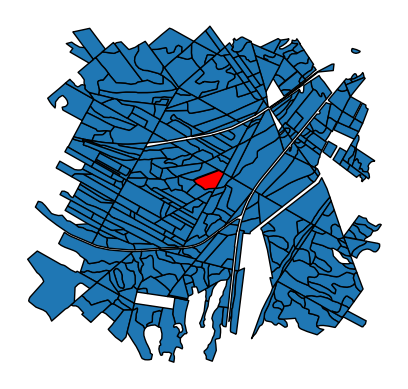
\includegraphics[width=.5\textwidth]{figures/andmestik/er_id_is10124223.png}
    \caption{Näidis ühe lageraie päringust saadud ümbrus}
    \label{fig:umbrusexample}
\end{figure}

Polügoon on geomeetriline kujund, mis määratleb kindla ala, ühendades üksteisega
punktid, et moodustada suletud piirjoon. Andmetöötluse ja ruumiandmete analüüsi
kontekstis kasutatakse polügoone, et täpselt määratleda geograafilisi alasid. \cite{WhatLocationPolygon}



\begin{figure}[H]
    \centering
    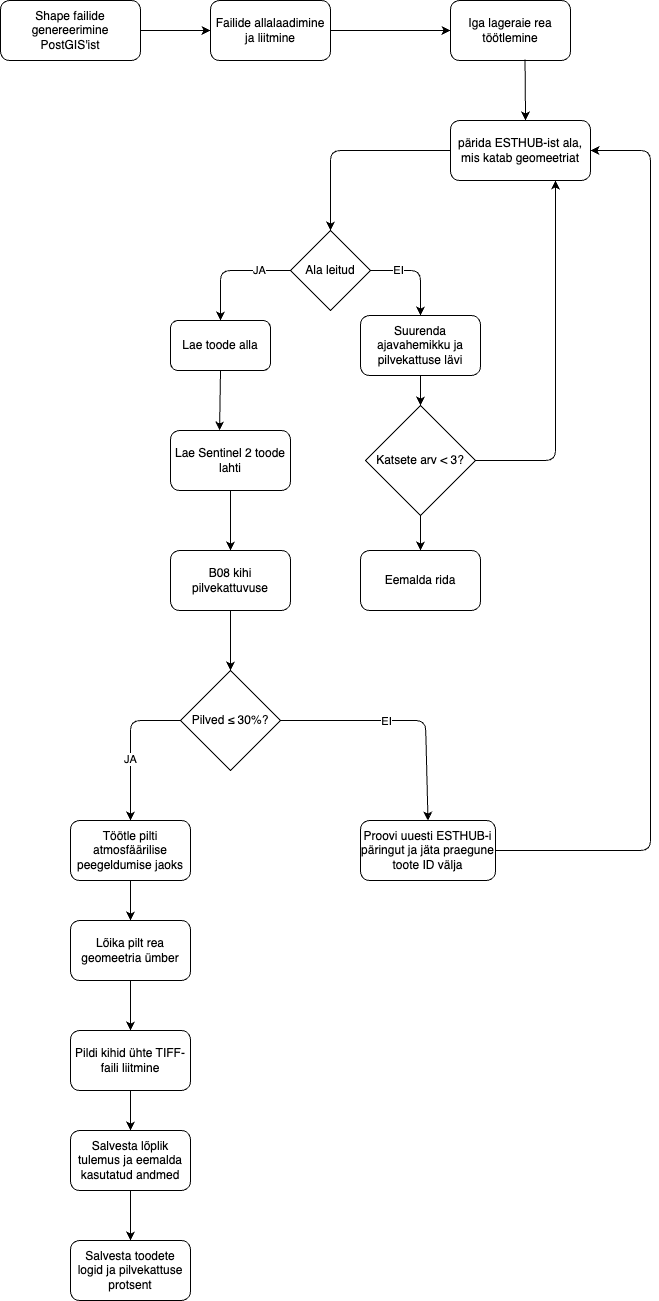
\includegraphics[width=.8\textwidth]{figures/andmestik/andmete_voog.drawio.png}
    \caption{Andmestiku loomise töövoog}
    \label{fig:terveflow}
\end{figure}


\section{Alusmudeli ülevaade}
Alustemudelid (\textit{Foundation models}) on suuremahulistel andmekogudel
ennastjuhendavalt treenitud sügavad närvivõrgud, mis toimivad üldotstarbelise
baasina mitmesuguste masinõppeülesannete lahendamiseks. Erinevalt
traditsioonilistest mudelitest, mis on välja töötatud konkreetse ülesande jaoks
ja nõuavad eraldi treeningut, on alus mudelid eelnevalt ettevalmistatud laia
valiku ülesannete sooritamiseks --- alates loomulikust keele töötlemisest ja
tekstigeneratsioonist kuni pildiklassifitseerimise ja vastuste genereerimiseni
--- ilma täiendava märgendatud õppematerjalita. Nende mudelite
kohanemisvõime tuleneb nii suurest parameetrite hulgast kui ka enesekontrollil
põhinevast õppestrateegiast, mis võimaldab neid hõlpsasti peenhäälestada
konkreetsete rakenduste jaoks, vähendades oluliselt arendusaja ja
arvutusressursside vajadust võimaldades keskenduda pigem mudeli peenhäälestusele kui treenimisele nullist. 
\cite{WhatAreFoundation}

\textbf{DINO v2} on Meta AI poolt välja töötatud \textit{Vision
Transformer}'itel (ViT) põhinevad isejuhitavat (self‑supervised, SSL) õppemeetodit, mille
ülesanne on genereerida üldotstarbelisi visuaalseid omadusi ilma märgendatud
treeningandmeteta. Mudeli struktuuri südameks on õpetaja--õpilase skeem, kus
õpilasmudeli parameetreid koheldakse tavalise ViT‑võrguna, aga õpetajamudeli
kaale uuendatakse õpilase kaalude eksponentsiaalse libiseva keskmise kaudu.
Treeningprotsessi stabiliseerimiseks ja tunnusruumi hajutamiseks on lisatud
Kozachenko--Leonenko (KoLeo) regulaarija, mis soodustab tunnuste ühtlast jaotust.
Õppetöö lõpus suurendatakse sisendpiltide resolutsiooni
ajutiselt 518\(\times \)518 pikslile, et parandada piksli tasemel
ülesannete, näiteks semantilise segmenteerimise ja objekti tuvastus ennustuse,
täpsust. Praktikas saavutab DINO v2 tänu optimeeritud
FlashAttention‑i ja PyTorch Full‑Sharded Data Parallel (FSDP) meetodile kuni
kahekordse kiiruse ning kolmekordse mälu tarbe vajaduse, võrreldes varasemate SSL‑mudelitega. \cite{oquabDINOv2LearningRobust2024}

\section{Treenimis protsetuurid}
Describe the training process, including parameter tuning (grid search, cross-validation), and optimization methods.